\section{Thiết kế nối trục}
Chọn vật liệu chốt - thép C45 với ứng suất uốn cho phép $[\sigma_F] = 70MPa$, ứng suất dập giữa chốt và ống $[\sigma_d] = 3MPa$. \\ 
Sử dụng nối trục đàn hồi theo yêu cầu của bài toán với các thông số như sau:\\
Momen truyền qua nối trục: T = 385,5 Nm \\
Đường kính trục $d_2 = 45mm$\\
\begin{figure}[H]
    \centering
    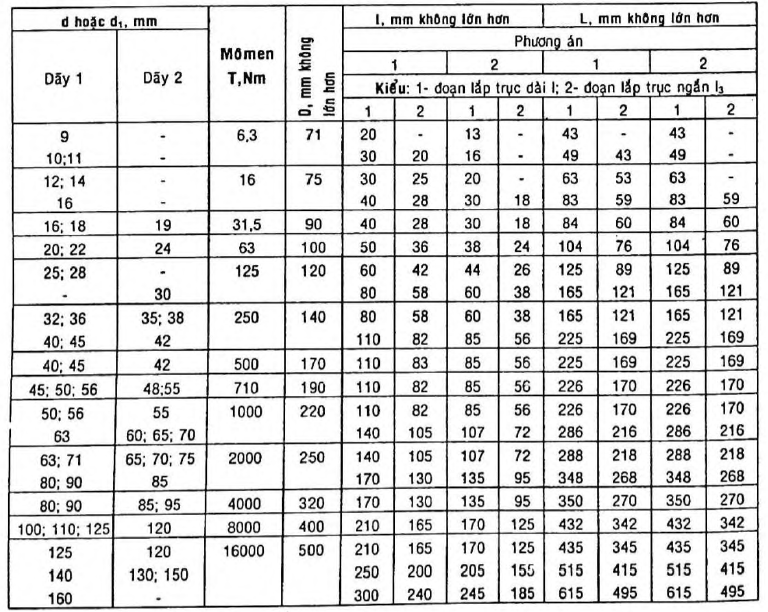
\includegraphics[width=0.8\textwidth]{pictures/noitruc.png}
    \caption{Các kích thước chính chọn nối trục vòng đàn hồi}
\end{figure}
\begin{figure}[H]
    \centering
    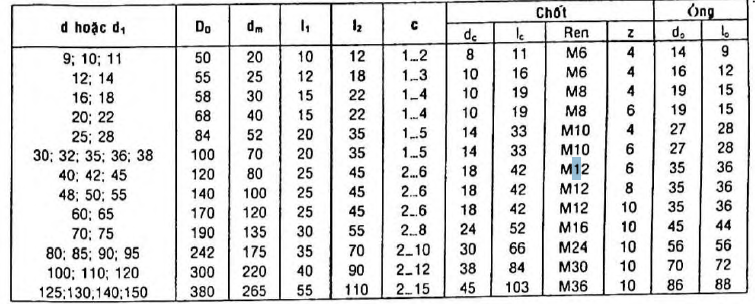
\includegraphics[width=0.8\textwidth]{pictures/noitruc2.png}
    \caption{Các kích thước phụ chọn nối trục vòng đàn hồi}
\end{figure}
Theo phụ lục ta chọn nối trục đàn hồi có: 
\begin{center}
\begin{tabular}{|c|c|c|c|c|c|c|c|c|c|c|c|}
    \hline
    d & $D_0 $  & $d_m$  & $l_1$  & $l_2$  & C  & $d_c$  & $l_c$  & Ren  & z  & $d_0$  & $l_0$ \\
    \hline
    45 & 120 & 80 & 25 & 45 & 3 & 18 & 42 & M12 & 6 & 35 & 36 \\
    \hline
\end{tabular}
\end{center}
Chọn vật liệu chốt thép C45 với ứng suất uốn cho phép, ứng suất trượt giữa chốt 
và ống là $[\sigma_d] =3MPa$ \\
Theo bảng 14.1 chọn chế độ làm việc K = 1,5.
\begin{figure}[H]
    \centering
    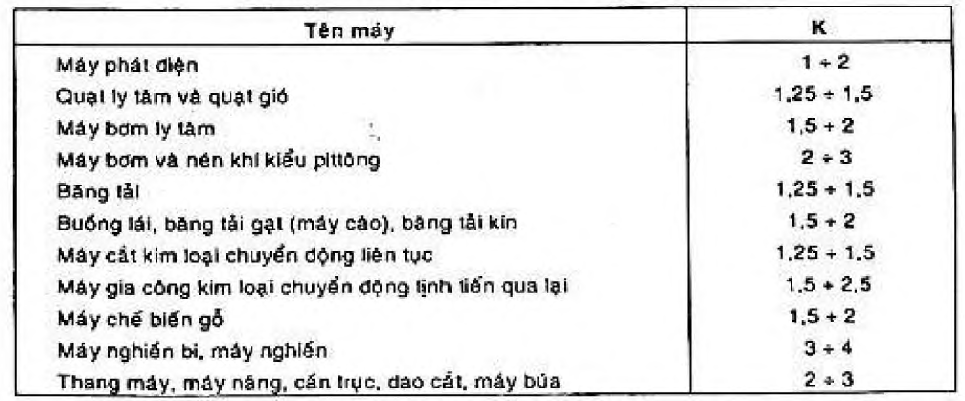
\includegraphics[width=1\textwidth]{pictures/hesolamviec.png}
    \caption{Hệ số làm việc K}
\end{figure}

Kiểm tra độ bền uốn:
\[
    \sigma_F = \frac{32KT.10^3.l_c}{\pi d_c^3.D_0.z} = \frac{32.1,5.385,5.10^3.42}{\pi.18^3.120.6} = 58,9MPa < [\sigma_F] = 70MPa
\]
\hspace*{0,82cm}Kiểm tra độ bền dập:
\[
    \sigma_d = \frac{2KT.10^3}{z.D_0.d_c.l_0}  = \frac{2.1,5.385,5.10^3}{6.120.18.36} = 2,48MPa < [\sigma_d] = 3MPa
\]
$\Rightarrow$ Thỏa mãn điều kiện bền uốn và bền dập.
\cleardoublepage